\documentclass{article}[18pt]
\ProvidesPackage{format}
%Page setup
\usepackage[utf8]{inputenc}
\usepackage[margin=0.7in]{geometry}
\usepackage{parselines} 
\usepackage[english]{babel}
\usepackage{fancyhdr}
\usepackage{titlesec}
\hyphenpenalty=10000

\pagestyle{fancy}
\fancyhf{}
\rhead{Sam Robbins}
\rfoot{Page \thepage}

%Characters
\usepackage{amsmath}
\usepackage{amssymb}
\usepackage{gensymb}
\newcommand{\R}{\mathbb{R}}

%Diagrams
\usepackage{pgfplots}
\usepackage{graphicx}
\usepackage{tabularx}
\usepackage{relsize}
\pgfplotsset{width=10cm,compat=1.9}
\usepackage{float}

%Length Setting
\titlespacing\section{0pt}{14pt plus 4pt minus 2pt}{0pt plus 2pt minus 2pt}
\newlength\tindent
\setlength{\tindent}{\parindent}
\setlength{\parindent}{0pt}
\renewcommand{\indent}{\hspace*{\tindent}}

%Programming Font
\usepackage{courier}
\usepackage{listings}
\usepackage{pxfonts}

%Lists
\usepackage{enumerate}
\usepackage{enumitem}

% Networks Macro
\usepackage{tikz}


% Commands for files converted using pandoc
\providecommand{\tightlist}{%
	\setlength{\itemsep}{0pt}\setlength{\parskip}{0pt}}
\usepackage{hyperref}

% Get nice commands for floor and ceil
\usepackage{mathtools}
\DeclarePairedDelimiter{\ceil}{\lceil}{\rceil}
\DeclarePairedDelimiter{\floor}{\lfloor}{\rfloor}

% Allow itemize to go up to 20 levels deep (just change the number if you need more you madman)
\usepackage{enumitem}
\setlistdepth{20}
\renewlist{itemize}{itemize}{20}

% initially, use dots for all levels
\setlist[itemize]{label=$\cdot$}

% customize the first 3 levels
\setlist[itemize,1]{label=\textbullet}
\setlist[itemize,2]{label=--}
\setlist[itemize,3]{label=*}

% Definition and Important Stuff
% Important stuff
\usepackage[framemethod=TikZ]{mdframed}

\newcounter{theo}[section]\setcounter{theo}{0}
\renewcommand{\thetheo}{\arabic{section}.\arabic{theo}}
\newenvironment{important}[1][]{%
	\refstepcounter{theo}%
	\ifstrempty{#1}%
	{\mdfsetup{%
			frametitle={%
				\tikz[baseline=(current bounding box.east),outer sep=0pt]
				\node[anchor=east,rectangle,fill=red!50]
				{\strut Important};}}
	}%
	{\mdfsetup{%
			frametitle={%
				\tikz[baseline=(current bounding box.east),outer sep=0pt]
				\node[anchor=east,rectangle,fill=red!50]
				{\strut Important:~#1};}}%
	}%
	\mdfsetup{innertopmargin=10pt,linecolor=red!50,%
		linewidth=2pt,topline=true,%
		frametitleaboveskip=\dimexpr-\ht\strutbox\relax
	}
	\begin{mdframed}[]\relax%
		\centering
		}{\end{mdframed}}



\newcounter{lem}[section]\setcounter{lem}{0}
\renewcommand{\thelem}{\arabic{section}.\arabic{lem}}
\newenvironment{defin}[1][]{%
	\refstepcounter{lem}%
	\ifstrempty{#1}%
	{\mdfsetup{%
			frametitle={%
				\tikz[baseline=(current bounding box.east),outer sep=0pt]
				\node[anchor=east,rectangle,fill=blue!20]
				{\strut Definition};}}
	}%
	{\mdfsetup{%
			frametitle={%
				\tikz[baseline=(current bounding box.east),outer sep=0pt]
				\node[anchor=east,rectangle,fill=blue!20]
				{\strut Definition:~#1};}}%
	}%
	\mdfsetup{innertopmargin=10pt,linecolor=blue!20,%
		linewidth=2pt,topline=true,%
		frametitleaboveskip=\dimexpr-\ht\strutbox\relax
	}
	\begin{mdframed}[]\relax%
		\centering
		}{\end{mdframed}}
\lhead{Software Methodologies - Computer Graphics}


\begin{document}
\begin{center}
\underline{\huge GPU Programming with WebGL}
\end{center}
\begin{definition}[Polygon model/mesh]
Comprises a set of connected polygons to represent an object
\end{definition}
\section{Why WebGL}
\begin{itemize}
	\item Cross-platform, browser-based
	\item Hardware-based rendering
	\item Support programmable rendering pipeline
	\item Zero setup effort before you start programming
\end{itemize}
\section{GPU Programming}
GPU
\begin{itemize}
	\item Typically comprises of hundreds to thousands of processors
	\item Process graphics primitives in parallel
\end{itemize}
Programmable rendering pipeline
\begin{itemize}
	\item Vertex shader and fragment shader are programmable
	\item GPU programming is also called shader programming
\end{itemize}
\section{Programmable rendering pipeline}
\begin{center}
	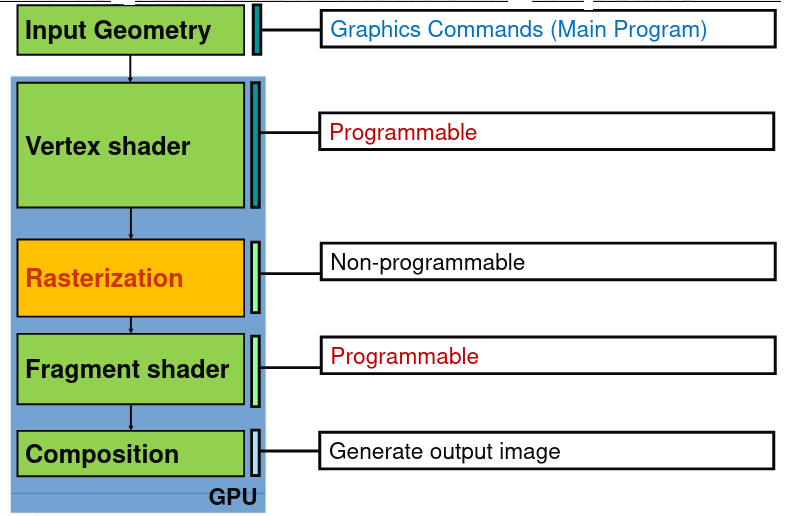
\includegraphics[scale=0.7]{pipeline}
\end{center}
Pixels - Colour info\\
Fragment - Single point with more information than a pixel, e.g.  lighting effects
\section{Shaders}
Vertex shader:
\begin{itemize}
	\item Manipulates per-vertex data such as vertex coordinates, normals, colors, and texture coordinates
\end{itemize}
Fragment shader:
\begin{itemize}
	\item Deals with surface points for processing
	\item Main goal: calculate colour for each pixel that will display on the screen
\end{itemize}
Rasterization process:
\begin{itemize}
	\item A black box (non programmable) generates fragments from outputs of vertex shader
\end{itemize}
\section{Data Structures}
\begin{definition}[Vertex Buffer Objects (VBOs)]
Contain the data that WebGL requires to describe the geometry that is going to be rendered
\end{definition}

\begin{definition}[Index Buffer Objects (IBOs)]
	Contain integers that use as references pointing to data in VBOs, in order to enable the reuse of the same vertex
\end{definition}

Attributes, uniforms and varyings are the three types of variables that you will find when programming with shaders
\begin{definition}[Attributes]
	Input variables used in the vertex shader (dynamic)
\end{definition}

\begin{definition}[Uniforms]
Input variables available for the vertex shader and the fragment shader (static)
\end{definition}

\begin{definition}[Varyings]
Used for passing data from the vertex shader to the fragment shader
\end{definition}








\end{document}